\begin{quote}
\textbf{Félix Guattari}: Imagine a fenced field in which there are
horses wearing adjustable blinkers, and let's say that the ``coefficient
of transversality'' will be precisely the adjustment of the blinkers. If
the horses are completely blind, a certain kind of traumatic encounter
will be produced. As soon as the blinkers are opened, one can imagine
that the horses will move about in a more harmonious way.
(\href{http://nine.fibreculturejournal.org/}{Quoted by Andrew Murphy},
himself quoting Gary Genosko)
\end{quote}

\begin{center}
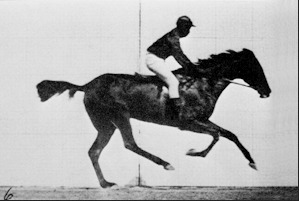
\includegraphics[width=.85\textwidth]{../pictures/horse.jpg}
\end{center}

From a design point of view: we should be conscious of interfaces that
are ``too loud'', and think about how that is compensated for by
isolation of various forms. With a too-narrow focus, collaboration is
impossible. However, with an overly-wide focus, things are chaotic in
other ways (see
\href{http://peeragogy.org/practice/antipatterns/co-learning-messy-with-lurkers/}{Co-Learning:
Messy with Lurkers}).

This anti-pattern sometimes goes by the name \emph{Not Invented Here}.
Many projects that are ostensibly oriented towards ``the commons''
nevertheless want to funnel participants into ``their way'' of thinking
about things. Be careful with that. Learning how to manage the
uncertainty that comes with experimentation is part of what makes the
postmodern organization tick! (See also:
\href{http://peeragogy.org/antipatterns/navel-gazing/}{Navel Gazing}.)
